\section{Learning \& Training Dynamics}

\subsection*{\textcolor{primaryteal}{Q: What is the role of Batch Normalization (BN) in training neural networks?}}
\textbf{Batch Normalization} normalizes the input of each layer to have zero mean and unit variance across a mini-batch. This reduces internal co-variate shift (changes in the distribution of layer inputs during training caused by the changing distribution of the previous layers), speeds up convergence, and stabilizes activation distributions and gradients.

\textbf{Mathematical Formulation}: For a mini-batch $B$ of size $m$:
\[
	\mu_B = \frac{1}{m} \sum_{i=1}^{m} x_i, \quad \sigma_B^2 = \frac{1}{m} \sum_{i=1}^{m} (x_i - \mu_B)^2
\]
\[
	\hat{x}_i = \frac{x_i - \mu_B}{\sqrt{\sigma_B^2 + \epsilon}}, \quad y_i = \gamma \hat{x}_i + \beta
\]
where $\epsilon$ is a small constant for numerical stability, and $\gamma, \beta$ are learnable parameters.

\subsection*{\textcolor{primaryteal}{Q: Why are learnable scale and shift parameters ($\gamma, \beta$) included in BN?}}
BN restricts the distribution of outputs into the same fixed distribution (mean=0, variance=1), which prevents the network from learning the optimal scale and bias. These parameters allow the network to undo the normalization if necessary, preserving representational power after the input is normalized.

\textbf{Parameter Learning}: The parameters $\gamma$ and $\beta$ are learned during training:
\[
	\gamma = \text{Var}[x]^{1/2}, \quad \beta = \mathbb{E}[x]
\]
This allows the network to recover the original distribution if it's optimal for the task.

\subsection*{\textcolor{primaryteal}{Q: Where should BN be applied in a neural network?}}
\textbf{Batch Normalization} is typically applied after the affine transformation (like a linear or convolutional layer) and before the activation function such as ReLU. BN normalizes the pre-activation values which stabilizes the distribution before they pass through nonlinearities, which keeps gradients flowing smoothly during backpropagation. BN, typically, is not applied to the output layers.

\textbf{Reasoning}: BN should normalize the inputs to activation functions, as activations like ReLU are sensitive to input distribution shifts. Normalizing pre-activations ensures the activation function receives well-distributed inputs.

\subsection*{\textcolor{primaryteal}{Q: What are the limitations of BN with small batch sizes?}}
Small batch sizes lead to noisy estimates of the mean and variance, which can destabilize training and degrade performance. This may result in issues such as batch-wise overfitting or jittery parameter updates. Additionally, Batch Normalization loses much of its regularization effect when batch statistics become unreliable. In practice, a "small batch" typically refers to fewer than 32 samples per batch per device.

\textbf{Statistical Analysis}: The variance of the batch statistics scales as $\text{Var}[\mu_B] = \frac{\sigma^2}{m}$, so smaller batches lead to noisier estimates.

\subsection*{\textcolor{primaryteal}{Q: How does batch normalization work during inference?}}
During inference, batch normalization (BN) uses the running averages of the mean and variance computed during training, rather than calculating them from the current batch of data. This ensures deterministic outputs regardless of batch size. However, the outputs during inference may differ slightly from those during training due to the shift from batch-wise statistics to running estimates.

\textbf{Running Statistics Update}: The running statistics are updated during training as:
\[
	\mu_{\text{running}} \leftarrow \alpha \mu_{\text{running}} + (1-\alpha) \mu_B
\]
\[
	\sigma^2_{\text{running}} \leftarrow \alpha \sigma^2_{\text{running}} + (1-\alpha) \sigma^2_B
\]
where $\alpha$ is typically 0.9 or 0.99.

\subsection*{\textcolor{primaryteal}{Q: How do BatchNorm, LayerNorm, GroupNorm, and InstanceNorm compare?}}
\begin{figure}[H]
	\centering
	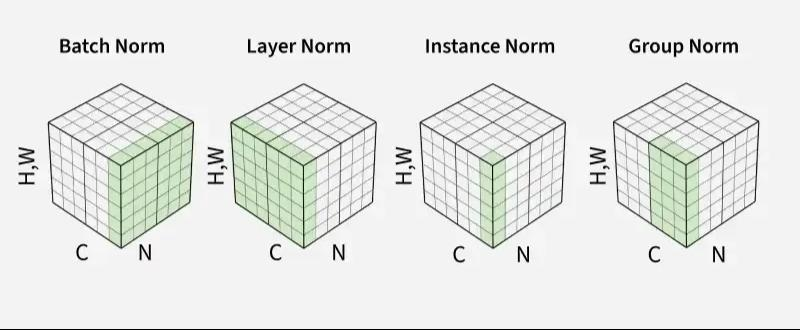
\includegraphics[width=0.8\textwidth]{images/norms.jpg}
	\caption{Source: \textit{https://www.geeksforgeeks.org/deep-learning/what-is-group-normalization/}}
\end{figure}

\begin{itemize}
	\item \textbf{Batch Normalization (BatchNorm)}: BatchNorm normalizes inputs across the batch dimension for each feature channel. It works well with large batch sizes and helps stabilize and accelerate training, but it can perform poorly with small batches and behaves differently during inference.

	\item \textbf{Layer Normalization (LayerNorm)}: LayerNorm normalizes across all feature dimensions within a single data sample. It is independent of batch size (robust for small batches) and is commonly used in architectures like Transformers and RNNs, but it tends to be less effective in convolutional neural networks.

	\item \textbf{Group Normalization (GroupNorm)}: GroupNorm divides channels into smaller groups and normalizes within each group. It performs consistently regardless of batch size and is particularly effective for convolutional models, though it requires tuning the number of groups (e.g., num groups=32).

	\item \textbf{Instance Normalization (InstanceNorm)}: InstanceNorm normalizes each individual sample and channel across spatial dimensions. It is widely used in style transfer applications as it helps remove instance-specific contrast information, but it may hurt performance in classification tasks where style information is important.
\end{itemize}

\textbf{Summary}: The choice of normalization method depends heavily on the task and batch size. For convolutional neural networks (CNNs) trained on large datasets like ImageNet, \textbf{BatchNorm} is the preferred choice. In scenarios with small batch sizes, such as object detection or segmentation, \textbf{GroupNorm} is typically more stable and effective. For natural language processing (NLP) and Transformer-based architectures, \textbf{LayerNorm} is widely used due to its batch-size independence. Finally, in style transfer or generative adversarial networks (GANs), \textbf{InstanceNorm} is favored for its ability to discard contrast and style-specific information.

\subsection*{\textcolor{primaryteal}{Q: What are the differences between SGD and Adam?}}
\textbf{SGD (Stochastic Gradient Descent)} uses a fixed or scheduled learning rate and is memory-efficient. The update rule is:
\[
	\theta_{t+1} = \theta_t - \eta_t \nabla_\theta J(\theta_t)
\]
where $\eta_t$ is the learning rate at step $t$.

\textbf{Adam (Adaptive Moment Estimation)} adapts learning rates for each parameter and converges faster but may overfit. It maintains exponential moving averages of gradients and squared gradients:
\[
	m_t = \beta_1 m_{t-1} + (1-\beta_1) \nabla_\theta J(\theta_t)
\]
\[
	v_t = \beta_2 v_{t-1} + (1-\beta_2) (\nabla_\theta J(\theta_t))^2
\]
\[
	\hat{m}_t = \frac{m_t}{1-\beta_1^t}, \quad \hat{v}_t = \frac{v_t}{1-\beta_2^t}
\]
\[
	\theta_{t+1} = \theta_t - \frac{\eta}{\sqrt{\hat{v}_t} + \epsilon} \hat{m}_t
\]

\textbf{Key Insight}: Adam typically converges faster but may generalize less well than SGD with proper learning rate scheduling.

\subsection*{\textcolor{primaryteal}{Q: What is the role of momentum in SGD?}}
\textbf{Momentum} accumulates past gradients to smooth updates and accelerate convergence, especially in consistent gradient directions, and dampen oscillations caused by noisy gradients.

\textbf{Mathematical Formulation}: The momentum update rule is:
\[
	v_{t+1} = \mu v_t - \eta \nabla_\theta J(\theta_t)
\]
\[
	\theta_{t+1} = \theta_t + v_{t+1}
\]
where $\mu$ is the momentum coefficient (typically 0.9).

\textbf{Benefits of Momentum}:
\begin{itemize}
	\item Accelerating convergence in consistent gradient directions
	\item Reducing oscillations in narrow valleys
	\item Improving training stability
	\item Helping escape local minima
\end{itemize}

\subsection*{\textcolor{primaryteal}{Q: What are advanced optimization techniques beyond Adam?}}
Several advanced optimizers have been developed to address limitations of Adam:

\begin{itemize}
	\item \textbf{AdamW}: Decouples weight decay from gradient-based updates (directly shrinks the weights after each update), leading to better generalization
	\item \textbf{RAdam}: Rectifies the variance of adaptive learning rates, providing more stable training
	\item \textbf{Lion}: Uses sign-based updates with momentum, achieving competitive performance with fewer parameters
	\item \textbf{AdaBelief}: Adapts step sizes based on belief in observed gradients, improving convergence
\end{itemize}

\subsection*{\textcolor{primaryteal}{Q: How can overfitting be reduced in machine learning?}}
Overfitting occurs when a model learns the training data too well, including noise, leading to poor generalization. Several techniques can help:

\begin{itemize}
	\item \textbf{Regularization}: Adding penalty terms to the loss function
	\item \textbf{Early Stopping}: Monitoring validation performance and stopping when it degrades
	\item \textbf{Data Augmentation}: Creating additional training examples through transformations
	\item \textbf{Dropout}: Randomly deactivating neurons during training
	\item \textbf{Cross-validation}: Using multiple train/validation splits to train a set of models and then select the appropriate model by comparing with the average performance of the models
\end{itemize}

\subsection*{\textcolor{primaryteal}{Q: What is the difference between L1 and L2 regularization?}}
Both L1 and L2 regularization add penalty terms to prevent overfitting, but they have different effects:

\textbf{L1 Regularization (Lasso)}: Adds $\lambda \sum_{i=1}^{n} |w_i|$ to the loss function
\begin{itemize}
	\item Promotes sparsity by driving some weights to exactly zero
	\item Useful for feature selection
	\item Less robust to outliers
\end{itemize}

\textbf{L2 Regularization (Ridge)}: Adds $\lambda \sum_{i=1}^{n} w_i^2$ to the loss function
\begin{itemize}
	\item Prevents any weight from becoming too large
	\item More robust to outliers
	\item All features contribute to the model
\end{itemize}

\subsection*{\textcolor{primaryteal}{Q: What is weight decay and how does it differ from L2 regularization?}}
\textbf{Weight decay} is a regularization technique that directly reduces the magnitude of weights during optimization, helping prevent overfitting by keeping weights small.

\textbf{Mathematical Formulation}: Weight decay adds a penalty term to the loss function:
\[
	L_{\text{total}} = L_{\text{original}} + \frac{\lambda}{2} \sum_{i=1}^{n} w_i^2
\]
where $\lambda$ is the weight decay coefficient.

\textbf{Key Differences from L2 Regularization}:
\begin{itemize}
	\item \textbf{Implementation}: Weight decay is typically implemented as a separate term in the optimizer, while L2 regularization is added to the loss function
	\item \textbf{Effect on gradients}: Weight decay directly reduces weights after each update, while L2 regularization affects gradients during backpropagation
	\item \textbf{Optimizer compatibility}: Weight decay works better with adaptive optimizers like Adam, while L2 regularization can interfere with their adaptive learning rates
\end{itemize}

\textbf{Benefits}:
\begin{itemize}
	\item \textbf{Better generalization}: Prevents weights from becoming too large
	\item \textbf{Improved training stability}: Helps maintain reasonable weight magnitudes
	\item \textbf{Reduced overfitting}: Limits model capacity effectively
	\item \textbf{Optimizer compatibility}: Works well with modern adaptive optimizers
\end{itemize}

\textbf{Implementation in Different Optimizers}:
\begin{itemize}
	\item \textbf{SGD}: Weight decay is equivalent to L2 regularization
	\item \textbf{Adam}: Weight decay is decoupled from gradient-based updates (AdamW)
	\item \textbf{AdamW}: Implements weight decay correctly by applying it after the adaptive update
\end{itemize}

\textbf{Tuning Guidelines}:
\begin{itemize}
	\item \textbf{Typical values}: $\lambda$ ranges from $10^{-6}$ to $10^{-2}$
	\item \textbf{Start small}: Begin with $10^{-4}$ and adjust based on validation performance
	\item \textbf{Monitor overfitting}: Increase if training loss is much lower than validation loss
	\item \textbf{Task-dependent}: Image classification typically uses $10^{-4}$, while language models may use $10^{-2}$
\end{itemize}

\subsection*{\textcolor{primaryteal}{Q: How does dropout work?}}
\textbf{Dropout} is a regularization technique that randomly sets a fraction of neurons to zero during training:

\begin{itemize}
	\item During training: Each neuron is dropped with probability $p$ (typically 0.5)
	\item During inference: All neurons are active, but weights are scaled by $(1-p)$
	\item Effect: Prevents co-adaptation of neurons and improves generalization
\end{itemize}

\subsection*{\textcolor{primaryteal}{Q: Why does dropout improve generalization?}}
Dropout improves generalization through several mechanisms:

\begin{itemize}
	\item \textbf{Prevents Co-adaptation}: Neurons cannot rely on specific combinations of other neurons
	\item \textbf{Ensemble Effect}: Each forward pass uses a different subnetwork, creating an implicit ensemble
	\item \textbf{Regularization}: Forces the network to be robust to missing information
	\item \textbf{Reduces Overfitting}: Limits the network's capacity to memorize training data
\end{itemize}

\subsection*{\textcolor{primaryteal}{Q: What are common activation functions and when to use them?}}
\begin{figure}[H]
	\centering
	\includegraphics[width=1\textwidth]{images/activation.png}
	\caption{Common activation functions and their properties}
\end{figure}

\textbf{Mathematical Formulations (Chronological Evolution)}:

\textbf{Sigmoid}: $\sigma(x) = \frac{1}{1 + e^{-x}}$
\begin{itemize}
	\item Outputs values between 0 and 1, useful for binary classification
	\item Derivative: $\sigma'(x) = \sigma(x)(1 - \sigma(x))$
	\item Suffers from vanishing gradients for extreme values
	\item Historical: One of the earliest activation functions, inspired by biological neurons
\end{itemize}

\textbf{Tanh}: $\tanh(x) = \frac{e^x - e^{-x}}{e^x + e^{-x}} = 2\sigma(2x) - 1$
\begin{itemize}
	\item Outputs values between -1 and 1, zero-centered, better for hidden layers
	\item Derivative: $\tanh'(x) = 1 - \tanh^2(x)$
	\item Better gradient flow than sigmoid due to zero-centering
	\item Historical: Improved upon sigmoid by addressing the zero-centering issue
\end{itemize}

\textbf{Softmax}: $\text{softmax}(x_i) = \frac{e^{x_i}}{\sum_{j=1}^{n} e^{x_j}}$
\begin{itemize}
	\item Outputs probability distribution, used in multi-class classification
	\item Ensures $\sum_{i=1}^{n} \text{softmax}(x_i) = 1$
	\item Numerically stable when using log-space computation
	\item Historical: Developed for multi-class classification and probability modeling
\end{itemize}

\textbf{ReLU}: $\text{ReLU}(x) = \max(0, x)$
\begin{itemize}
	\item Most popular, computationally efficient, helps with vanishing gradients
	\item Derivative: $\text{ReLU}'(x) = \begin{cases} 1 & \text{if } x > 0 \\ 0 & \text{if } x \leq 0 \end{cases}$
	\item Can suffer from "dying ReLU" problem: neurons that always output 0 due to negative inputs, becoming permanently inactive
	\item Historical: Revolutionized deep learning by solving vanishing gradient problem
\end{itemize}

\textbf{Leaky ReLU}: $\text{LeakyReLU}(x) = \begin{cases} x & \text{if } x > 0 \\ \alpha x & \text{if } x \leq 0 \end{cases}$
\begin{itemize}
	\item Addresses dying ReLU problem by allowing small negative gradients
	\item Derivative: $\text{LeakyReLU}'(x) = \begin{cases} 1 & \text{if } x > 0 \\ \alpha & \text{if } x \leq 0 \end{cases}$
	\item Typical $\alpha = 0.01$
	\item Historical: First attempt to fix the dying ReLU problem
\end{itemize}

\textbf{ELU}: $\text{ELU}(x) = \begin{cases} x & \text{if } x > 0 \\ \alpha(e^x - 1) & \text{if } x \leq 0 \end{cases}$
\begin{itemize}
	\item Smooth activation function that outputs negative values for negative inputs
	\item Derivative: $\text{ELU}'(x) = \begin{cases} 1 & \text{if } x > 0 \\ \text{ELU}(x) + \alpha & \text{if } x \leq 0 \end{cases}$
	\item Typical $\alpha = 1.0$, ensures output approaches $-\alpha$ for large negative inputs
	\item Better gradient flow than ReLU and helps with vanishing gradients
	\item Historical: Introduced smoothness and negative outputs to address ReLU limitations
\end{itemize}

\textbf{GELU}: $\text{GELU}(x) = x \cdot \Phi(x)$
\begin{itemize}
	\item Smooth approximation of ReLU, used in modern architectures
	\item Where $\Phi(x)$ is the cumulative distribution function of standard normal
	\item Approximated as: $\text{GELU}(x) \approx 0.5x(1 + \tanh(\sqrt{2/\pi}(x + 0.044715x^3)))$
	\item Historical: Developed for transformer architectures, provides smooth gradients
\end{itemize}

\textbf{Swish}: $\text{Swish}(x) = x \cdot \sigma(x)$
\begin{itemize}
	\item Self-gated activation, often outperforms ReLU
	\item Derivative: $\text{Swish}'(x) = \sigma(x) + x \cdot \sigma(x)(1 - \sigma(x))$
	\item Smooth, non-monotonic function with learnable parameters
	\item Historical: Discovered through automated search, showing better performance than ReLU
\end{itemize}

\textbf{GLU}: $\text{GLU}(x) = (W_1x + b_1) \odot \sigma(W_2x + b_2)$
\begin{itemize}
	\item Gated mechanism that controls information flow through the network
	\item Where $\odot$ denotes element-wise multiplication (Hadamard product)
	\item The gate $\sigma(W_2x + b_2)$ controls how much of $(W_1x + b_1)$ passes through
	\item Used in transformer architectures and language models
	\item Historical: Introduced gating mechanisms for better information control
\end{itemize}

\textbf{SwiGLU}: $\text{SwiGLU}(x) = (W_1x + b_1) \odot \text{Swish}(W_2x + b_2)$
\begin{itemize}
	\item Combines GLU with Swish activation for the gate
	\item Mathematical formulation: $\text{SwiGLU}(x) = (W_1x + b_1) \odot (W_2x + b_2) \cdot \sigma(W_2x + b_2)$
	\item Often outperforms standard GLU and is used in modern LLMs like PaLM and LLaMA
	\item Provides better gradient flow and training stability than ReLU-based gates
	\item Historical: Latest evolution, combining the best of GLU and Swish for modern LLMs
\end{itemize}

\subsection*{\textcolor{primaryteal}{Q: What are activation functions?}}
\textbf{Activation functions} are non-linear transformations applied to the output of neurons in neural networks. They introduce non-linearity into the network, enabling it to learn complex patterns and relationships in data.

\textbf{Key purposes}:
\begin{itemize}
	\item \textbf{Non-linearity}: Without activation functions, neural networks would only be able to represent linear transformations
	\item \textbf{Gradient flow}: They control how gradients flow during backpropagation
	\item \textbf{Output range}: They determine the range of values that neurons can output
	\item \textbf{Feature learning}: Different activations help learn different types of features
\end{itemize}

\textbf{Mathematical role}: For a neuron with input $z$, the activation function $f$ produces output $a = f(z)$, where $f$ is typically differentiable to enable gradient-based learning.

\subsection*{\textcolor{primaryteal}{Q: How to choose the right activation functions?}}
\textbf{Choosing activation functions} depends on the specific task, network architecture, and training dynamics:

\textbf{For hidden layers}:
\begin{itemize}
	\item \textbf{ReLU}: Default choice for most deep networks due to computational efficiency and good gradient flow
	\item \textbf{Leaky ReLU/ELU}: Use when you want to avoid dying ReLU problem
	\item \textbf{GELU/Swish}: Better for transformer architectures and when smooth gradients are important
	\item \textbf{Tanh}: Good for RNNs and when you need bounded outputs
\end{itemize}

\textbf{For output layers}:
\begin{itemize}
	\item \textbf{Sigmoid}: Binary classification (outputs 0-1 probabilities)
	\item \textbf{Softmax}: Multi-class classification (outputs probability distribution)
	\item \textbf{Linear}: Regression tasks (unbounded outputs)
	\item \textbf{ReLU}: When outputs should be non-negative
\end{itemize}

\textbf{Considerations}:
\begin{itemize}
	\item \textbf{Vanishing gradients}: Avoid sigmoid/tanh in deep networks
	\item \textbf{Computational cost}: ReLU is fastest, GELU/Swish are more expensive
	\item \textbf{Task requirements}: Match output range to task needs
	\item \textbf{Architecture compatibility}: Some activations work better with specific architectures
\end{itemize}

\subsection*{\textcolor{primaryteal}{Q: When should you use Sigmoid vs Softmax?}}
The choice between Sigmoid and Softmax depends on the task:

\textbf{Sigmoid}: Use for binary classification or when you need independent probabilities
\begin{itemize}
	\item Outputs values between 0 and 1
	\item Each output is independent of others
	\item Suitable for multi-label classification
\end{itemize}

\textbf{Softmax}: Use for multi-class classification when outputs should sum to 1
\begin{itemize}
	\item Outputs probability distribution that sums to 1
	\item Outputs are dependent (compete with each other)
	\item Suitable for single-label classification
\end{itemize}

\subsection*{\textcolor{primaryteal}{Q: What is gradient flow and why is it important?}}
\textbf{Gradient flow} refers to how gradients propagate backward through the network during training:

\begin{itemize}
	\item \textbf{Vanishing Gradients}: Gradients become very small in deep networks, slowing learning
	\item \textbf{Exploding Gradients}: Gradients become very large, causing unstable training
	\item \textbf{Importance}: Proper gradient flow is essential for training deep networks effectively
\end{itemize}

\textbf{Solutions}:
\begin{itemize}
	\item Proper weight initialization
	\item Batch normalization
	\item Residual connections
	\item Careful choice of activation functions
\end{itemize}

\subsection*{\textcolor{primaryteal}{Q: What are advanced weight initialization strategies?}}
Proper weight initialization is crucial for training deep networks:

\begin{itemize}
	\item \textbf{Xavier/Glorot}: Scales weights by $\sqrt{\frac{2}{n_{in} + n_{out}}}$ for sigmoid/tanh
	\item \textbf{He}: Scales weights by $\sqrt{\frac{2}{n_{in}}}$ for ReLU activations
	\item \textbf{Orthogonal}: Initializes weights as orthogonal matrices, preserving gradient norms
	\item \textbf{LSUV}: Layer-sequential unit-variance initialization for better training dynamics
\end{itemize}

\subsection*{\textcolor{primaryteal}{Q: What are curriculum learning and learning rate scheduling?}}
\textbf{Curriculum learning} presents training examples in a meaningful order, starting with simpler examples and gradually increasing difficulty.

\textbf{Mathematical Formulation}: For a curriculum function \(c(t)\) that determines difficulty at step \(t\):
\[
	\text{Difficulty}(t) = c(t) \cdot \text{MaxDifficulty}
\]

\textbf{Learning Rate Scheduling} adjusts the learning rate during training:
\begin{itemize}
	\item \textbf{Step Decay}: Reduces learning rate by a factor every N epochs
	\item \textbf{Exponential Decay}: Continuously decreases learning rate exponentially
	\item \textbf{Cosine Annealing}: Smoothly decreases learning rate following cosine curve
	\item \textbf{One Cycle}: Increases then decreases learning rate in a single cycle
\end{itemize}

\subsection*{\textcolor{primaryteal}{Q: What are advanced regularization techniques?}}
Beyond L1/L2 and dropout, several advanced regularization techniques exist:

\begin{itemize}
	\item \textbf{Label Smoothing}: Replaces hard labels with soft probability distributions
	\item \textbf{Mixup}: Creates new training examples by interpolating between pairs
	\item \textbf{CutMix}: Combines parts of different images for data augmentation
	\item \textbf{Stochastic Depth}: Randomly drops entire layers during training
	\item \textbf{ShakeDrop}: Applies random scaling to residual connections
\end{itemize}

\textbf{Mathematical Benefits}:
\begin{itemize}
	\item Improved generalization through better calibration
	\item Enhanced robustness to adversarial examples
	\item Better handling of label noise
	\item Reduced overfitting in deep networks
\end{itemize}

\subsection*{\textcolor{primaryteal}{Q: How do Precision-Recall curves and ROC curves compare, and when should each be used?}}
\begin{center}
	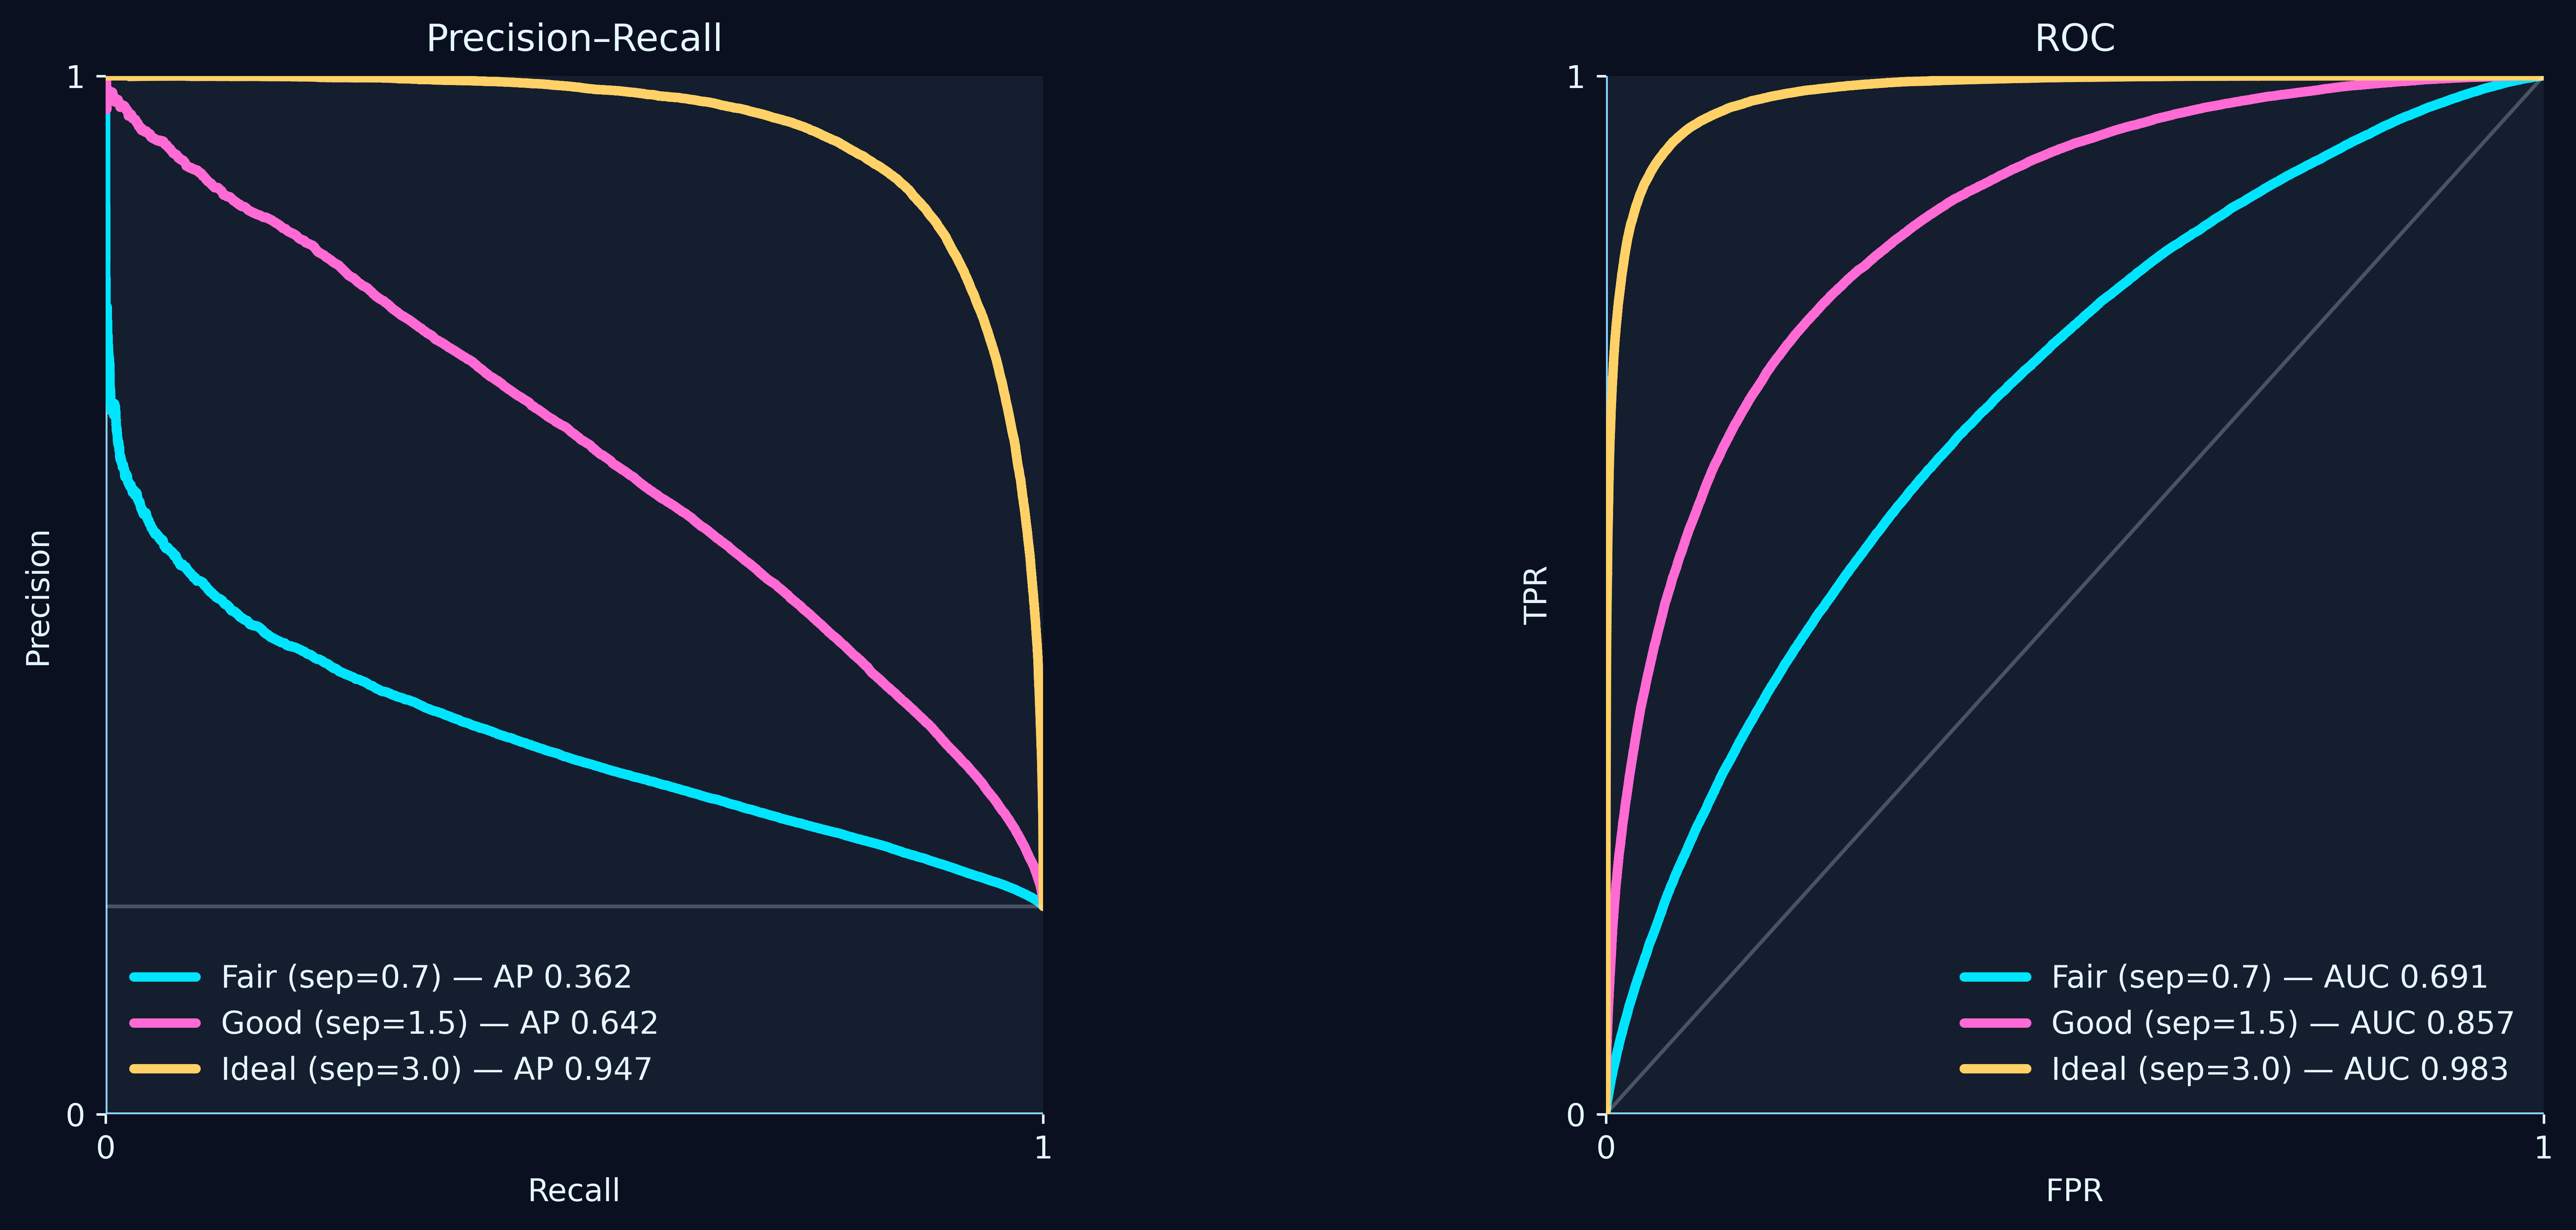
\includegraphics[width=0.6\textwidth]{images/pr_roc.png}
\end{center}

\textbf{Precision-Recall Curve}:
Focus on the positive class performance and are more informative for imbalanced datasets. More sensitive to the positive class distribution.
\begin{itemize}
	\item \textbf{Precision}: $P = \frac{TP}{TP + FP}$ (positive predictive value)
	\item \textbf{Recall}: $R = \frac{TP}{TP + FN}$ (sensitivity, true positive rate)
	\item \textbf{F1-Score}: $F1 = 2 \cdot \frac{P \cdot R}{P + R}$ (harmonic mean)
\end{itemize}

\textbf{ROC Curve}:
Show the trade-off between TPR and FPR across all thresholds. More stable and less sensitive to the positive class distribution.
\begin{itemize}
	\item \textbf{True Positive Rate (TPR)}: $TPR = \frac{TP}{TP + FN}$ (same as recall)
	\item \textbf{False Positive Rate (FPR)}: $FPR = \frac{FP}{FP + TN}$
	\item \textbf{AUC-ROC}: Area under the ROC curve, measures overall discriminative ability
\end{itemize}

\textbf{When to Use Each}:

\textbf{Precision-Recall Curves are preferable when}:
\begin{itemize}
	\item \textbf{Class imbalance exists} (especially when negative class dominates)
	\item \textbf{Positive class is rare} (e.g., fraud detection, medical diagnosis)
	\item \textbf{False positives are costly} (e.g., spam detection, medical screening)
	\item \textbf{You care about the positive class performance} more than overall accuracy
\end{itemize}

\textbf{ROC Curves are preferable when}:
\begin{itemize}
	\item \textbf{Classes are relatively balanced}
	\item \textbf{You want to evaluate overall discriminative ability}
	\item \textbf{Both false positives and false negatives have similar costs}
	\item \textbf{You need a threshold-independent measure of performance}
\end{itemize}

\textbf{Imbalanced Dataset Considerations}:
In highly imbalanced datasets where the negative class dominates (e.g., 95\% negative, 5\% positive):

\begin{itemize}
	\item \textbf{PR curves} provide more meaningful insights because they focus on the minority class
	\item \textbf{ROC curves} can be misleading, showing good performance even when the model struggles with the positive class
	\item \textbf{High precision} becomes crucial to avoid overwhelming users with false positives
	\item \textbf{Recall} must be balanced against precision based on business requirements
\end{itemize}

\textbf{Practical Guidelines}:
\begin{itemize}
	\item \textbf{Use PR curves} for imbalanced datasets, rare event detection, and when positive class performance is critical
	\item \textbf{Use ROC curves} for balanced datasets and when you need overall discriminative ability
	\item \textbf{Always consider both} when evaluating models to get a complete picture
	\item \textbf{Choose thresholds} based on business requirements (precision vs. recall trade-off)
\end{itemize}


